Data processing is an important part of many studies. Type and size of data as well as the type of processing justifies the processing method. In seismological studies mostly we are dealing with numerical data with different customized processing. In many cases, user write a function in a programming language (e.g. MATLAB\textsuperscript{\textregistered}, Python, C, Fortran) and process the data. Regarding the type of data and processing, we may have many steps of processing data in a project. Also we may need to change a parameter and repeat the processing different times.  Writing down the processing steps is a good practice to avoid confusion, keep track of the processing, and be able to return back and look for the probable bugs in case of wrong results. However, since it is not automated, you my unwillingly skip one step of processing. Even with complete documentation, in the case of finding the problem in processing step, you need to repeat the whole process and go through the whole steps. Developing a data analysis package could be an excellent alternative to apply customized processing functions on massive data sets. In this short note, I present how to develop a data processing package. This note is not about methods of data processing, or getting and cleaning data. Obviously, there are many different approach to tackle the problem. If you have  scripts in a different programming language and you are using those scripts repeatedly to process data, you may find this document helpful. Shell scripts (e.g. Unix shell) are robust computer program for handling files and folders. In this short note, I explain how to use shell scripts to mange the input and output file, also report any problem during the processing. The core function could be written in any programming language. Since, bringing MATLAB\textsuperscript{\textregistered} in unix platform needs extra steps, also many people use MATLAB\textsuperscript{\textregistered} for daily data processing, the examples are based on MATLAB\textsuperscript{\textregistered}. The method is applicable to other programming languages, with the difference that they don't have complexity of calling MATLAB\textsuperscript{\textregistered} in the Unix platform.

Shell script is preparing a data with a correct format and correct name at the right time to the core function and receive the results at the right time and pass to other program or archive it.

\begin{figure} [ht]
\centering
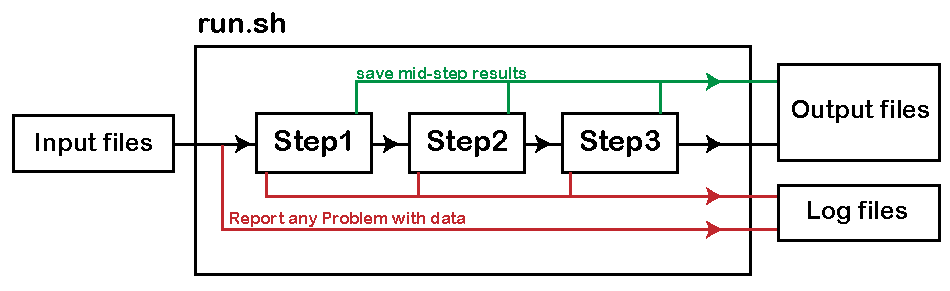
\includegraphics[scale=0.6]{figures/pdf/Figure01.pdf} 
\caption{Relative path of folders.}
\label{fig:structure}
\end{figure}